% A circular diagram of a TeX workflow
% Author: Stefan Kottwitz
% https://www.packtpub.com/hardware-and-creative/latex-cookbook
\documentclass[]{standalone}
\usepackage{tikz} 
\usetikzlibrary{shapes,arrows}
\usetikzlibrary{calc}
%\usepgfplotslibrary{external} 
%\tikzexternalize 
\usepackage{sansmath}
\sansmath


\tikzstyle{block} = [rectangle, draw, 
text width=8em, text centered, rounded corners, minimum height=4em]
\tikzstyle{line} = [draw, -latex']

\begin{document}
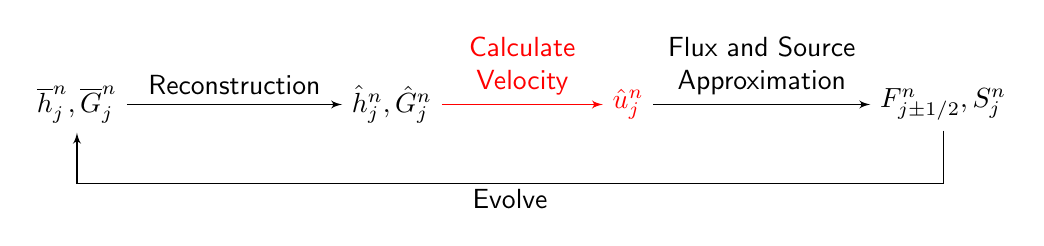
\begin{tikzpicture} 
\fontfamily{cmss}
 \node (PP) {$\overline{h}^n_j,\overline{G}^n_j$};
 \node [right of=PP, node distance=4cm](MM) {$\hat{h}^n_j,\hat{G}^n_j$};
 \node [color=red,right of= MM, node distance=3cm](CP) {$\hat{u}^n_j$};
 \node [right of= CP, node distance=4cm](CC) {$F^{n}_{j\pm 1/2}, S^n_j$};
 \path [line] (PP) -> (MM) node[pos=0.5,above,sloped] {Reconstruction};
 \path [color=red,line] (MM) -> (CP) node[pos=0.5,above,sloped, align=center] {Calculate \\ Velocity};
 \path [line] (CP) -> (CC) node[pos=0.5,above,sloped, align=center] {Flux and Source \\ Approximation};
 \path [line] (CC) -- ($ (CC) + (0,-1) $) --  ($ (PP) + (0,-1) $) ->  (PP) ;
 \node (a) at ($(MM)  + (0,-1.2) $){};
 \node (b) at ($(CP)  + (0,-1.2) $){};
 \node at ($(a)!0.5!(b)$) {Evolve};
 %\path [line] (CP) -> (PP) node[pos=0.5,above,sloped] {Finite Volume};
\end{tikzpicture} 
\end{document}